\documentclass{article}
\usepackage[utf8]{inputenc}
\usepackage{tikz}
\usepackage{amsmath}
\usepackage{pgfplots}


\title{LaTeX for GHP Presentation}
\author{Edwin Trejo}
\date{June 2022}

\begin{document}

\maketitle

\section{Introduction}



Imaginary numbers are multiples of the imaginary unit, \(i\), defined as:
\[\sqrt{-1}=i\]

Combining an imaginary number with a real number gives a complex number, which has the form: \[z=x+iy\]
Where \(i\) is the imaginary unit, and \(x\) and \(y\) are real numbers
 
\[Re(Z) = x \ \ \ \ \ \ \ \  Im(Z) = y\]

A complex number can be graphed on the complex plane by replacing the x- and y- axes of the 
cartesian plane with the real and imaginary axes
\newline

\[(x,y) \rightleftharpoons z = x + iy\]

\[C(t) = (cos(t), sin(t)) \rightleftharpoons C(t) = cos(t) + isin(t)\]
\newline


\newpage
\[C(t) = cos(t) + isin(t)\]
\begin{center}
    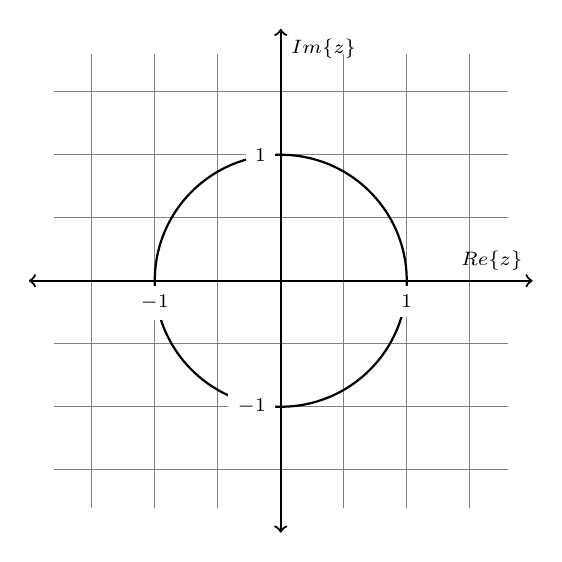
\begin{tikzpicture}[scale=1.6]
        \begin{scope}[thick,font=\scriptsize]
        % Axes:
        % Are simply drawn using line with the `->` option to make them arrows:
        % The main labels of the axes can be places using `node`s:
        \draw[
            step=.5cm,
            gray,
            very thin
            ] 
            (-1.8,-1.8) grid (1.8,1.8);
        \draw [<->] (-2,0) -- (2,0) node [above left]  {$Re\{z\}$};
        \draw [<->] (0,-2) -- (0,2) node [below right] {$Im\{z\}$};
    
        \draw[thick] (0cm,0cm) circle(1.0cm);
        
        %x-ticks
    \foreach \x/\xtext in {-1, 1}
    \draw (\x cm,1pt) -- (\x cm,-1pt) node[
                    anchor=north,
                    fill=white
                    ] 
                    {$\xtext$};
    %y-ticks
    \foreach \y/\ytext in {-1, 1}
    \draw (1pt,\y cm) -- (-1pt,\y cm) node[
                    anchor=east,
                    fill=white
                    ] 
                    {$\ytext$};
    
        \end{scope}
    \end{tikzpicture}
    \end{center}


    \[C(t) = (cos(t), sin(t))\]
    \begin{center}
        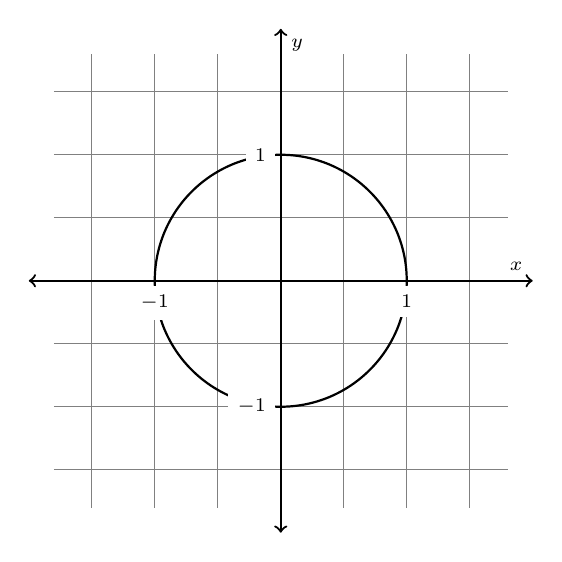
\begin{tikzpicture}[scale=1.6]
            \begin{scope}[thick,font=\scriptsize]
            % Axes:
            % Are simply drawn using line with the `->` option to make them arrows:
            % The main labels of the axes can be places using `node`s:
            \draw[
                step=.5cm,
                gray,
                very thin
                ] 
                (-1.8,-1.8) grid (1.8,1.8);
            \draw [<->] (-2,0) -- (2,0) node [above left]  {$x$};
            \draw [<->] (0,-2) -- (0,2) node [below right] {$y$};
        
            \draw[thick] (0cm,0cm) circle(1.0cm);
            
            %x-ticks
        \foreach \x/\xtext in {-1, 1}
        \draw (\x cm,1pt) -- (\x cm,-1pt) node[
                        anchor=north,
                        fill=white
                        ] 
                        {$\xtext$};
        %y-ticks
        \foreach \y/\ytext in {-1, 1}
        \draw (1pt,\y cm) -- (-1pt,\y cm) node[
                        anchor=east,
                        fill=white
                        ] 
                        {$\ytext$};
        
            \end{scope}
        \end{tikzpicture}
        \end{center}
        

\newpage
        \[e^{i(\alpha)} = cos(\alpha) + isin(\alpha)\]
\begin{center}
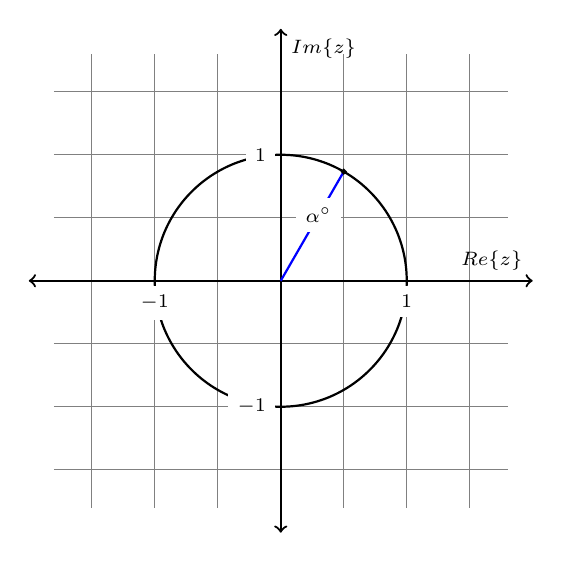
\begin{tikzpicture}[scale=1.6]
    \begin{scope}[thick,font=\scriptsize]
    % Axes:
    % Are simply drawn using line with the `->` option to make them arrows:
    % The main labels of the axes can be places using `node`s:
    \draw[
        step=.5cm,
        gray,
        very thin
        ] 
        (-1.8,-1.8) grid (1.8,1.8);
    \draw [<->] (-2,0) -- (2,0) node [above left]  {$Re\{z\}$};
    \draw [<->] (0,-2) -- (0,2) node [below right] {$Im\{z\}$};

    \draw[thick] (0cm,0cm) circle(1.0cm);

    \foreach \x in {60} {
                % lines from center to point
                \draw[blue] (0cm,0cm) -- (\x:1cm);
                % dots at each point
                \filldraw[black] (\x:1cm) circle(0.4pt);
                % draw each angle in degrees
                \draw (\x:0.6cm) node[fill=white] {$\alpha^\circ$};
        }
    
    %x-ticks
\foreach \x/\xtext in {-1, 1}
\draw (\x cm,1pt) -- (\x cm,-1pt) node[
                anchor=north,
                fill=white
                ] 
                {$\xtext$};
%y-ticks
\foreach \y/\ytext in {-1, 1}
\draw (1pt,\y cm) -- (-1pt,\y cm) node[
                anchor=east,
                fill=white
                ] 
                {$\ytext$};

    \end{scope}
\end{tikzpicture}
\end{center}


\[e^{i(\alpha + \beta)} = cos(\alpha + \beta) + isin(\alpha + \beta)\]
\begin{center}
    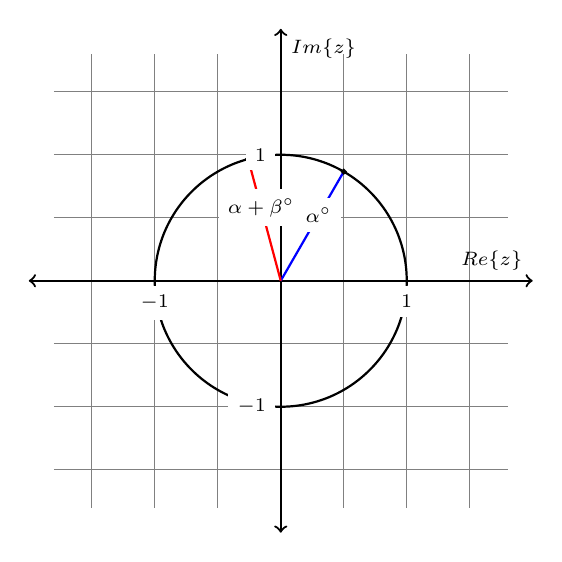
\begin{tikzpicture}[scale=1.6]
        \begin{scope}[thick,font=\scriptsize]
        % Axes:
        % Are simply drawn using line with the `->` option to make them arrows:
        % The main labels of the axes can be places using `node`s:
        \draw[
            step=.5cm,
            gray,
            very thin
            ] 
            (-1.8,-1.8) grid (1.8,1.8);
        \draw [<->] (-2,0) -- (2,0) node [above left]  {$Re\{z\}$};
        \draw [<->] (0,-2) -- (0,2) node [below right] {$Im\{z\}$};
    
        \draw[thick] (0cm,0cm) circle(1.0cm);
    
        \foreach \x in {60} {
                % lines from center to point
                \draw[blue] (0cm,0cm) -- (\x:1cm);
                % dots at each point
                \filldraw[black] (\x:1cm) circle(0.4pt);
                % draw each angle in degrees
                \draw (\x:0.6cm) node[fill=white] {$\alpha^\circ$};
        }

        \foreach \x in {105} {
                % lines from center to point
                \draw[red] (0cm,0cm) -- (\x:1cm);
                % dots at each point
                \filldraw[black] (\x:1cm) circle(0.4pt);
                % draw each angle in degrees
                \draw (\x:0.6cm) node[fill=white] {$\alpha + \beta^\circ$};
        }

        
        %x-ticks
    \foreach \x/\xtext in {-1, 1}
    \draw (\x cm,1pt) -- (\x cm,-1pt) node[
                    anchor=north,
                    fill=white
                    ] 
                    {$\xtext$};
    %y-ticks
    \foreach \y/\ytext in {-1, 1}
    \draw (1pt,\y cm) -- (-1pt,\y cm) node[
                    anchor=east,
                    fill=white
                    ] 
                    {$\ytext$};
    
        \end{scope}
    \end{tikzpicture}
\end{center}


\newpage
\[f(t) = sin(t)\]
\newline
\[f'(t) = cos(t)\]
\newline

\[f(t) = sin(t)\]
\[f'(t) = cos(t)\]
\[f''(t) = -sin(t)\]
\[f'''(t) = -cos(t)\]
\newline
\[f^4(t) = ?\]
\newline
\[f^4(t) = sin(t)\]
\newline

\[f(t) = \sum_{n=0}^{\infty} \frac{f^{(n)}(0)*t^n}{n!} \]
\newline
\newline
\[sin(t) = \sum_{n=0}^{\infty} \frac{(sin(0))^{(n)}*t^n}{n!} \]
\[\sum_{n=0}^{\infty} \frac{(sin(0))^{(n)}*t^n}{n!} = sin(0) + cos(0)t + \frac{-sin(0)t^2}{2!} + \frac{-cos(0)t^3}{3!} -+ ...\]
\[sin(t) = 0 + t - 0 - \frac{t^3}{3!} + ...\]
\[sin(t) = t - \frac{t^3}{3!} + \frac{t^5}{5!} - \frac{t^7}{7!} + ...\]
\newline
\[cos(t) = 1 - \frac{t^2}{2!} + \frac{t^4}{4!} - \frac{t^6}{6!} + ...\]
\newline
\newline

\[C(t) = (1 - \frac{t^2}{2!} + \frac{t^4}{4!} -+ ...) + i( t - \frac{t^3}{3!} + \frac{t^5}{5!} -+ ...)\]
\newline
\[C(t) = (1 + \frac{(it)^2}{2!} + \frac{(it)^4}{4!} + ...) + i(t + \frac{i^2t^3}{3!} + \frac{i^4t^5}{5!} + ...)\]
\newline
\[C(t) = (1 + \frac{(it)^2}{2!} + \frac{(it)^4}{4!} + ...) + (it + \frac{(it)^3}{3!} + \frac{(it)^5}{5!} + ...)\]
\newline
\[C(t) = 1 + it + \frac{(it)^2}{2!} + \frac{(it)^3}{3!} + \frac{(it)^4}{4!} + \frac{(it)^5}{5!} + ...\]


\[f(t) = e^t\]
\[f'(t) = e^t\]
\[f^{(n)}(t) = e^t\]
\newline
\[e^t = \sum_{n=0}^{\infty} \frac{[e^0]^{(n)} * t^n}{n!}\]
\[e^t = e^0 + e^0t + \frac{e^0t^2}{2!} + \frac{e^0t^3}{3!} + ...\]
\[e^t = 1 + t + \frac{t^2}{2!} + \frac{t^3}{3!} + \frac{t^4}{4!} + \frac{t^5}{5!} +...\]
\[e^{it} = 1 + it + \frac{(it)^2}{2!} + \frac{(it)^3}{3!} + \frac{(it)^4}{4!} + \frac{(it)^5}{5!} + ...\]
\newline
\[e^{it} = C(t)\]
\[e^{it} = (1 - \frac{t^2}{2!} + \frac{t^4}{4!} -+ ...) + i( t - \frac{t^3}{3!} + \frac{t^5}{5!} -+ ...)\]
\[e^{it} = cos(t) + isin(t)\]
\newline
\[e^{i\alpha} = cos(\alpha) + isin(\alpha)\]
\newline
\[e^{i(\alpha + \beta)} = cos(\alpha + \beta) + isin(\alpha + \beta)\] 
\[e^{i(\alpha + \beta)}\]
\[e^{i\alpha + i\beta}\]
\[e^{i\alpha} * e^{i\beta}\]





\end{document}